%\VignetteEngine{knitr::knitr}
%\VignetteIndexEntry{Grade of Membership Clustering and Visualization using CountClust}
%\VignettePackage{CountClust}

% To compile this document
% library('knitr'); rm(list=ls()); knit('CountClust/vignettes/count-clust.Rnw')
% library('knitr'); rm(list=ls()); knit2pdf('CountClust/vignettes/count-clust.Rnw'); openPDF('count-clust.pdf')
% !Rnw weave = knitr

\documentclass[12pt]{article}

\newcommand{\ecostructure}{\textit{ecostructure}}
\usepackage{dsfont}
\usepackage{cite}




\RequirePackage{/Library/Frameworks/R.framework/Versions/3.3/Resources/library/BiocStyle/resources/tex/Bioconductor}

\AtBeginDocument{\bibliographystyle{/Library/Frameworks/R.framework/Versions/3.3/Resources/library/BiocStyle/resources/tex/unsrturl}}



\bioctitle[\ecostructure{} - Grade of Membership Model and Visualization for ecological species abundance data]{\ecostructure{} - Grade of Membership Model and Visualization for ecological species abundance data}

\begin{document}

\maketitle

\section{Introduction}

The \textbf{ecostructure} package is an R package that replicates the statistical analysis in this paper, but its toolbox of functions is generic enough in handling and analyzing other species abundance data. The package provides functions for fitting the Grade of Membership (GoM) model, along with the visualization of model fit using Block Structure plot \ref{Pritchard}\ref{Taddy}. The package comes with the raw taxonomic data saved as an ExpressionSet object and provides a pipeline for reading and processing counts data corresponding to different dimensions of diversity, e.g. - phylogenetic, regional and functional, which serve as readymade input for the GoM model. This package is an upgraded version of the CountClust package due to Dey et al \ref{Dey} for fitting GoM models on RNA-seq data

\section{Installation}

The package is available on Github and can be installed as follows



\begin{knitrout}
\definecolor{shadecolor}{rgb}{0.969, 0.969, 0.969}\color{fgcolor}\begin{kframe}
\begin{alltt}
\hlkwd{library}\hlstd{(devtools)}
\hlkwd{install_github}\hlstd{(}\hlstr{"kkdey/ecostructure"}\hlstd{)}
\end{alltt}
\end{kframe}
\end{knitrout}

Load the package as

\begin{knitrout}
\definecolor{shadecolor}{rgb}{0.969, 0.969, 0.969}\color{fgcolor}\begin{kframe}
\begin{alltt}
\hlkwd{library}\hlstd{(ecostructure)}
\end{alltt}


{\ttfamily\noindent\color{warningcolor}{\#\# Warning: replacing previous import 'ape::rotate' by 'raster::rotate' when loading 'ecostructure'}}

{\ttfamily\noindent\color{warningcolor}{\#\# Warning: replacing previous import 'ape::zoom' by 'raster::zoom' when loading 'ecostructure'}}

{\ttfamily\noindent\color{warningcolor}{\#\# Warning: replacing previous import 'raster::density' by 'stats::density' when loading 'ecostructure'}}\begin{alltt}
\hlkwd{library}\hlstd{(Biobase)}
\end{alltt}
\end{kframe}
\end{knitrout}

to use the GoM model, the user needs to install the **maptpx** package

\begin{knitrout}
\definecolor{shadecolor}{rgb}{0.969, 0.969, 0.969}\color{fgcolor}\begin{kframe}
\begin{alltt}
\hlkwd{library}\hlstd{(devtools)}
\hlkwd{install_github}\hlstd{(}\hlstr{"kkdey/maptpx"}\hlstd{)}
\end{alltt}
\end{kframe}
\end{knitrout}


\section{Data Preparation}

One can load the taxonomic data, together with the grid metadata ans species metadata as an ExpressionSet object as follows

\begin{knitrout}
\definecolor{shadecolor}{rgb}{0.969, 0.969, 0.969}\color{fgcolor}\begin{kframe}
\begin{alltt}
\hlstd{data} \hlkwb{<-} \hlkwd{get}\hlstd{(}\hlkwd{load}\hlstd{(}\hlkwd{system.file}\hlstd{(}\hlstr{"extdata"}\hlstd{,} \hlstr{"HimalayanBirdsData.rda"}\hlstd{,}
                             \hlkwc{package} \hlstd{=} \hlstr{"ecostructure"}\hlstd{)))}
\hlstd{taxonomic_counts} \hlkwb{<-} \hlkwd{t}\hlstd{(}\hlkwd{exprs}\hlstd{(data))}
\hlstd{taxonomic_counts[}\hlnum{1}\hlopt{:}\hlnum{5}\hlstd{,}\hlnum{1}\hlopt{:}\hlnum{5}\hlstd{]}
\end{alltt}
\begin{verbatim}
##    Macropygia_unchall Streptopelia_chinensis Streptopelia_senegalensis
## A2                  0                      0                         0
## A3                  0                      0                         0
## A4                  0                      0                         0
## A6                  0                      0                         0
## A7                  0                      0                         0
##    Columba_pulchricollis Streptopelia_orientalis
## A2                     0                       0
## A3                     0                       0
## A4                     0                       0
## A6                     0                       0
## A7                     2                       0
\end{verbatim}
\end{kframe}
\end{knitrout}


The corresponding grid metadata can be read as

\begin{knitrout}
\definecolor{shadecolor}{rgb}{0.969, 0.969, 0.969}\color{fgcolor}\begin{kframe}
\begin{alltt}
\hlstd{grid_metadata} \hlkwb{<-} \hlkwd{pData}\hlstd{(}\hlkwd{phenoData}\hlstd{(data))}
\hlkwd{head}\hlstd{(grid_metadata)}
\end{alltt}
\begin{verbatim}
##    Elevation North East WorE
## A2       198  27.0 92.9    E
## A3       734  27.0 92.4    E
## A4      1243  27.0 92.4    E
## A6      2629  27.1 92.5    E
## A7      2340  27.1 92.4    E
## A8       300  27.0 93.0    E
\end{verbatim}
\end{kframe}
\end{knitrout}

The species metadata can be read as follows

\begin{knitrout}
\definecolor{shadecolor}{rgb}{0.969, 0.969, 0.969}\color{fgcolor}\begin{kframe}
\begin{alltt}
\hlstd{species_metadata} \hlkwb{<-} \hlkwd{pData}\hlstd{(}\hlkwd{featureData}\hlstd{(data))}
\hlkwd{head}\hlstd{(species_metadata)}
\end{alltt}
\begin{verbatim}
##                           bill_length bill_width bill_depth wing tarsus  mass
## Macropygia_unchall              11.08       4.26       4.97  198   26.3 168.0
## Streptopelia_chinensis          10.77       3.50       3.87  140   22.6 159.0
## Streptopelia_senegalensis        9.23       2.88       3.27  130   20.4  83.9
## Columba_pulchricollis           12.98       5.59       5.68  203   25.4 330.0
## Streptopelia_orientalis         10.88       4.09       3.90  192   25.5 233.0
## Chalcophaps_indica              11.77       3.61       4.42  151   26.3 121.0
\end{verbatim}
\end{kframe}
\end{knitrout}


Along with the taxonomic data and metadata, the package provides the phylogenetic tree data for the bird species as a **.tre** file that can be loaded as follows, using the package **ape**.

\begin{knitrout}
\definecolor{shadecolor}{rgb}{0.969, 0.969, 0.969}\color{fgcolor}\begin{kframe}
\begin{alltt}
\hlstd{phylo_tree} \hlkwb{<-} \hlstd{ape}\hlopt{::}\hlkwd{read.tree}\hlstd{(}\hlkwd{system.file}\hlstd{(}\hlstr{"extdata"}\hlstd{,} \hlstr{"AllHim_Mar_27_2015.tre"}\hlstd{,}
                             \hlkwc{package} \hlstd{=} \hlstr{"ecostructure"}\hlstd{))}
\end{alltt}


{\ttfamily\noindent\color{warningcolor}{\#\# Warning in ape::read.tree(system.file("{}extdata"{}, "{}AllHim\_Mar\_27\_2015.tre"{}, : empty character string.}}\begin{alltt}
\hlstd{phylo_tree}
\end{alltt}
\begin{verbatim}
## NULL
\end{verbatim}
\end{kframe}
\end{knitrout}


The shape files for the regional motif analysis can be loaded as follows

\begin{knitrout}
\definecolor{shadecolor}{rgb}{0.969, 0.969, 0.969}\color{fgcolor}\begin{kframe}
\begin{alltt}
\hlstd{shp_file} \hlkwb{<-} \hlstd{ape}\hlopt{::}\hlkwd{read.tree}\hlstd{(}\hlkwd{system.file}\hlstd{(}\hlstr{"extdata"}\hlstd{,} \hlstr{"AllHim_Mar_27_2015.tre"}\hlstd{,}
                             \hlkwc{package} \hlstd{=} \hlstr{"ecostructure"}\hlstd{))}
\end{alltt}


{\ttfamily\noindent\color{warningcolor}{\#\# Warning in ape::read.tree(system.file("{}extdata"{}, "{}AllHim\_Mar\_27\_2015.tre"{}, : empty character string.}}\begin{alltt}
\hlstd{shp_file}
\end{alltt}
\begin{verbatim}
## NULL
\end{verbatim}
\end{kframe}
\end{knitrout}

\section{Grade of Membership Model and Visualization}

Here we illustrate how one can fit the Grade of Membership model and perform the visualization of the model fit using the Block Structure plot. Here we present a case study with number of clusters chosen to be between $2$ and $4$.

\begin{knitrout}
\definecolor{shadecolor}{rgb}{0.969, 0.969, 0.969}\color{fgcolor}\begin{kframe}
\begin{alltt}
\hlstd{elevation_metadata}\hlkwb{=}\hlstd{grid_metadata}\hlopt{$}\hlstd{Elevation;}
\hlstd{east_west_dir} \hlkwb{=} \hlstd{grid_metadata}\hlopt{$}\hlstd{WorE;}
\hlstd{gom_fit} \hlkwb{<-} \hlstd{CountClust}\hlopt{::}\hlkwd{FitGoM}\hlstd{(taxonomic_counts,} \hlkwc{K}\hlstd{=}\hlnum{2}\hlopt{:}\hlnum{4}\hlstd{,} \hlkwc{tol}\hlstd{=}\hlnum{0.1}\hlstd{)}
\end{alltt}
\begin{verbatim}
## 
## Estimating on a 38 document collection.
## Fit and Bayes Factor Estimation for K = 2
## log posterior increase: 3789, 36.6, 0.7, 4.2, 51.7, done.
## log BF( 2 ) = 2192.15
## 
## Estimating on a 38 document collection.
## Fit and Bayes Factor Estimation for K = 3
## log posterior increase: 3568.5, 7.3, 43.3, 14, 57.9, 12.9, 0.2, done.
## log BF( 3 ) = 2448.06
## 
## Estimating on a 38 document collection.
## Fit and Bayes Factor Estimation for K = 4
## log posterior increase: 3535.7, 24.4, 89.4, 44, 1.3, 2.5, 64.8, 28.4, 0.9, 1.1, done.
## log BF( 4 ) = 2161.59
\end{verbatim}
\end{kframe}
\end{knitrout}


\begin{verb} gom_fit \end{verb} is a list of size 3, with each component representing the model fit for the cluster $k$, varying from 2 to 4. The two main components of the model fit are the membership proportion matrix $\omega$, given by \begin{verb} gom_fit[[k]]$omega \end{verb} and the motif matrix \begin{verb} gom_fit[[k]]$theta \end{verb}. Examples for $K=2$ are

\begin{knitrout}
\definecolor{shadecolor}{rgb}{0.969, 0.969, 0.969}\color{fgcolor}\begin{kframe}
\begin{alltt}
\hlstd{omega} \hlkwb{<-} \hlstd{gom_fit[[}\hlnum{2}\hlstd{]]}\hlopt{$}\hlstd{omega}
\hlkwd{head}\hlstd{(omega)}
\end{alltt}
\begin{verbatim}
##         topic
## document        1        2        3
##       A2 0.999819 9.66e-05 8.43e-05
##       A3 0.999357 5.47e-04 9.61e-05
##       A4 0.998530 1.25e-03 2.21e-04
##       A6 0.000143 9.99e-01 5.93e-04
##       A7 0.000110 9.99e-01 4.94e-04
##       A8 0.999736 9.35e-05 1.71e-04
\end{verbatim}
\begin{alltt}
\hlkwd{rowSums}\hlstd{(omega)}
\end{alltt}
\begin{verbatim}
## A2 A3 A4 A6 A7 A8 B1 B2 B3 B4 B5 D1 D3 G1 J1 J2 J4 J5 J6 K1 K2 K4 K5 K6 L1 M1 
##  1  1  1  1  1  1  1  1  1  1  1  1  1  1  1  1  1  1  1  1  1  1  1  1  1  1 
## M2 M3 M4 N1 N2 N3 S1 U3 U4 MA U1 U2 
##  1  1  1  1  1  1  1  1  1  1  1  1
\end{verbatim}
\begin{alltt}
\hlstd{theta} \hlkwb{<-} \hlstd{gom_fit[[}\hlnum{2}\hlstd{]]}\hlopt{$}\hlstd{theta}
\hlkwd{head}\hlstd{(theta)}
\end{alltt}
\begin{verbatim}
##                            topic
## phrase                             1        2        3
##   Macropygia_unchall        6.08e-07 2.05e-03 9.07e-07
##   Streptopelia_chinensis    7.27e-03 5.66e-07 7.03e-04
##   Streptopelia_senegalensis 3.32e-03 5.64e-07 9.06e-07
##   Columba_pulchricollis     6.08e-07 1.03e-03 9.06e-07
##   Streptopelia_orientalis   2.32e-03 6.38e-07 1.63e-02
##   Chalcophaps_indica        3.32e-03 5.65e-07 9.07e-07
\end{verbatim}
\begin{alltt}
\hlkwd{colSums}\hlstd{(theta)}
\end{alltt}
\begin{verbatim}
## 1 2 3 
## 1 1 1
\end{verbatim}
\end{kframe}
\end{knitrout}

Using the grid metadata, we provide a Block Structure Plot representation of the membership proportion matrix. In a block Structure plot representation, one metadata is used for forming blocks (here the East/West direction) and in each block, the
the samples (along the rows of the Structure plot) are arranged by a second metadata (say Elevation).

\begin{knitrout}
\definecolor{shadecolor}{rgb}{0.969, 0.969, 0.969}\color{fgcolor}\begin{kframe}
\begin{alltt}
\hlkwd{BlockStructure}\hlstd{(omega,} \hlkwc{blocker_metadata} \hlstd{= east_west_dir,}
               \hlkwc{order_metadata} \hlstd{= elevation_metadata,}
               \hlkwc{yaxis_label} \hlstd{=} \hlstr{"Elevation"}\hlstd{,}
               \hlkwc{levels_decreasing} \hlstd{=} \hlnum{FALSE}\hlstd{)}
\end{alltt}
\end{kframe}
\end{knitrout}


\begin{figure}[htp]
\begin{center}
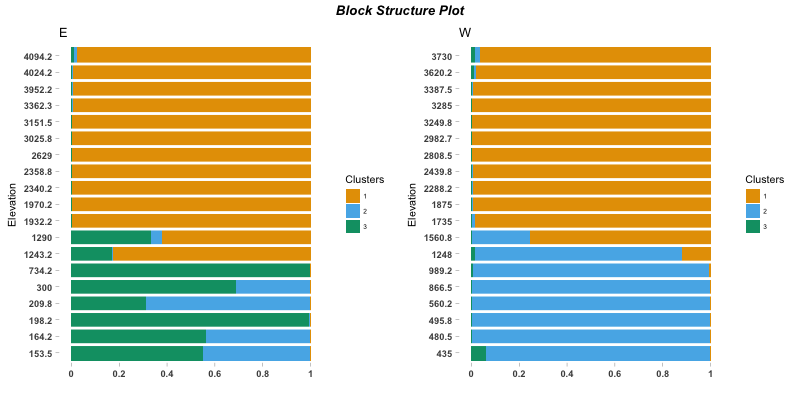
\includegraphics[width=6in,height=6in]{figure/block_structure.png}
\end{center}
\end{figure}

\newpage

\textbf{ecostructure} provides tools to compare the GoM model fit on the data with respect to null model using the \begin{verb} nullmodel_GoM \end{verb} function.

\begin{knitrout}
\definecolor{shadecolor}{rgb}{0.969, 0.969, 0.969}\color{fgcolor}\begin{kframe}
\begin{alltt}
\hlkwd{nullmodel_GoM}\hlstd{(taxonomic_counts,} \hlkwc{K}\hlstd{=}\hlnum{2}\hlstd{,}
               \hlkwc{tol}\hlstd{=}\hlnum{500}\hlstd{,} \hlkwc{null.model}\hlstd{=}\hlstr{"frequency"}\hlstd{,}
               \hlkwc{iter_randomized}\hlstd{=}\hlnum{5}\hlstd{,} \hlkwc{plot}\hlstd{=}\hlnum{FALSE}\hlstd{)}
\end{alltt}
\begin{verbatim}
## 
## Estimating on a 38 document collection.
## Fit and Bayes Factor Estimation for K = 2
## log posterior increase: 2945.2, done.
## log BF( 2 ) = 360.74
## 
## Estimating on a 38 document collection.
## Fit and Bayes Factor Estimation for K = 2
## log posterior increase: 3153.1, done.
## log BF( 2 ) = 406.06
## 
## Estimating on a 38 document collection.
## Fit and Bayes Factor Estimation for K = 2
## log posterior increase: 2741.2, done.
## log BF( 2 ) = 249.28
## 
## Estimating on a 38 document collection.
## Fit and Bayes Factor Estimation for K = 2
## log posterior increase: 2599.8, done.
## log BF( 2 ) = 391.53
## 
## Estimating on a 38 document collection.
## Fit and Bayes Factor Estimation for K = 2
## log posterior increase: 2570.9, done.
## log BF( 2 ) = 265.86
## 
## Estimating on a 38 document collection.
## Fit and Bayes Factor Estimation for K = 2
## log posterior increase: 3268.9, done.
## log BF( 2 ) = 1115.29
## $GoMBF.obs
## [1] 16076
## 
## $GoMBF.rand
## [1] 13376 12534 13173 13762 13191
## 
## $pval
## [1] 0
\end{verbatim}
\end{kframe}
\end{knitrout}

The function returns for a fixed $K$, the observed Bayes factor for the GoM model fit on the actual counts data, as well as the Bayes factor from applying GoM model on \begin{verb} iter_randomized \end{verb} many counts matrices generated under a specified null model. It also provdies a p-value of the observed Bayes factor with respect to the distribution of the Bayes factors from GoM on null model generated matrices.

In the above example \textbf{frequency} based null model was used. The other options are \textbf{richness}, \textbf{trialswap} and \textbf{independentswap}. Ideally if the observed Bayes factor should be higher than the Bayes factors from null model generated counts data.


\section{Processing motif data}

In this section, we demonstrate how \textbf{ecostructure} can be used to process
grid level counts data corresponding to different axes of diversity, that may range from being functional to regional to phylogenetic.

\subsection{phylogenetic motif}

For building the counts data corresponding to phylogenetic diversity, we provide a function,
\begin{verb} collapse_counts_by_phylo () \end{verb} to collapse the taxa in the taxonomic counts data based on the phylogenetic similarity profile of the species.
The function reads in the taxonomic counts data and the phylogenetic tree data and a user defined cut off at which to slice the tree and collapse the taxa in each branch into a single phylogenetic unit.

\begin{knitrout}
\definecolor{shadecolor}{rgb}{0.969, 0.969, 0.969}\color{fgcolor}\begin{kframe}
\begin{alltt}
\hlstd{tree} \hlkwb{<-} \hlstd{ape}\hlopt{::}\hlkwd{read.tree}\hlstd{(}\hlkwd{system.file}\hlstd{(}\hlstr{"extdata"}\hlstd{,}
                                   \hlstr{"grids_tree_3_10_16.tre"}\hlstd{,}
                                    \hlkwc{package} \hlstd{=} \hlstr{"ecostructure"}\hlstd{))}
\hlstd{phylo_counts} \hlkwb{<-} \hlkwd{collapse_counts_by_phylo}\hlstd{(taxonomic_counts,}
                                         \hlstd{tree,} \hlkwc{collapse_at} \hlstd{=} \hlnum{10}\hlstd{)}
\hlkwd{dim}\hlstd{(phylo_counts)}
\end{alltt}
\begin{verbatim}
## [1]  38 196
\end{verbatim}
\end{kframe}
\end{knitrout}

\subsection{regional motif}

For the regional profile, \textbf{ecostructure} allows the user to create Global assemblage dispersion fields and build maps data from those fields. To create the assemblage dispersion fields, the user would require to obatin the shapefiles (*.shp* files) for the all the species in the observed data.

One source of obtaining the *.shp* files for mapping to geographic boundaries is from the Natural Earth webpage (www.naturalearthdata.com/downloads). For our Himalyan birds data, we obatined the *.shp* files from BirdLife International (www.birdlife.org).

The user can put all the *.shp* files in the \begin{verb} all_bird_shapefiles () \end{verb} and then using this folder of shapefiles and the local taxonomic data, the user can create the global assemblage dispersion fields as follows

\begin{knitrout}
\definecolor{shadecolor}{rgb}{0.969, 0.969, 0.969}\color{fgcolor}\begin{kframe}
\begin{alltt}
\hlstd{disp} \hlkwb{<-} \hlkwd{CreateGlobalDispersionFields}\hlstd{(taxonomic_counts,}
              \hlkwc{shapefiles_dir} \hlstd{=} \hlstr{"all_bird_sjapefiles/"}\hlstd{)}
\end{alltt}
\end{kframe}
\end{knitrout}


\begin{knitrout}
\definecolor{shadecolor}{rgb}{0.969, 0.969, 0.969}\color{fgcolor}\begin{kframe}
\begin{alltt}
\hlstd{dispersion.field} \hlkwb{<-} \hlkwd{readRDS}\hlstd{(}\hlkwd{system.file}\hlstd{(}\hlstr{"extdata"}\hlstd{,}
                    \hlstr{"dispersion_field_list.rds"}\hlstd{,} \hlkwc{package} \hlstd{=} \hlstr{"ecostructure"}\hlstd{))}
\hlstd{proj} \hlkwb{<-} \hlkwd{CRS}\hlstd{(}\hlstr{' +proj=longlat +ellps=WGS84'}\hlstd{)}
\hlstd{global_shapefile} \hlkwb{<-} \hlkwd{readShapeLines}\hlstd{(}\hlkwd{system.file}\hlstd{(}\hlstr{"extdata"}\hlstd{,}
         \hlstr{"ne_50m_admin_0_countries/ne_50m_admin_0_countries.shp"}\hlstd{,}
          \hlkwc{package} \hlstd{=} \hlstr{"ecostructure"}\hlstd{),} \hlkwc{proj4string}\hlstd{=proj)}
\hlkwd{par}\hlstd{(}\hlkwc{mfrow} \hlstd{=} \hlkwd{c}\hlstd{(}\hlnum{1}\hlstd{,}\hlnum{1}\hlstd{))}
\hlstd{maps} \hlkwb{<-} \hlkwd{CreateMapsFromDispersionFields}\hlstd{(dispersion.field, global_shapefile)}
\end{alltt}
\end{kframe}
\end{knitrout}

The function returns a list of map plots with as many elements as the number of sites. We can see the maps as follows

\begin{knitrout}
\definecolor{shadecolor}{rgb}{0.969, 0.969, 0.969}\color{fgcolor}\begin{kframe}
\begin{alltt}
\hlstd{maps[[}\hlnum{1}\hlstd{]]}
\end{alltt}


{\ttfamily\noindent\color{warningcolor}{\#\# Warning in grid.Call(L\_textBounds, as.graphicsAnnot(x\$label), x\$x, x\$y, : font "{}Symbol"{} could not be found for family "{}"{}}}

{\ttfamily\noindent\color{warningcolor}{\#\# Warning in grid.Call(L\_textBounds, as.graphicsAnnot(x\$label), x\$x, x\$y, : font "{}Symbol"{} could not be found for family "{}"{}}}

{\ttfamily\noindent\color{warningcolor}{\#\# Warning in grid.Call(L\_textBounds, as.graphicsAnnot(x\$label), x\$x, x\$y, : font "{}Symbol"{} could not be found for family "{}"{}}}

{\ttfamily\noindent\color{warningcolor}{\#\# Warning in grid.Call(L\_textBounds, as.graphicsAnnot(x\$label), x\$x, x\$y, : font "{}Symbol"{} could not be found for family "{}"{}}}

{\ttfamily\noindent\color{warningcolor}{\#\# Warning in grid.Call(L\_textBounds, as.graphicsAnnot(x\$label), x\$x, x\$y, : font "{}Symbol"{} could not be found for family "{}"{}}}

{\ttfamily\noindent\color{warningcolor}{\#\# Warning in grid.Call(L\_textBounds, as.graphicsAnnot(x\$label), x\$x, x\$y, : font "{}Symbol"{} could not be found for family "{}"{}}}

{\ttfamily\noindent\color{warningcolor}{\#\# Warning in grid.Call(L\_textBounds, as.graphicsAnnot(x\$label), x\$x, x\$y, : font "{}Symbol"{} could not be found for family "{}"{}}}

{\ttfamily\noindent\color{warningcolor}{\#\# Warning in grid.Call(L\_textBounds, as.graphicsAnnot(x\$label), x\$x, x\$y, : font "{}Symbol"{} could not be found for family "{}"{}}}

{\ttfamily\noindent\color{warningcolor}{\#\# Warning in grid.Call(L\_textBounds, as.graphicsAnnot(x\$label), x\$x, x\$y, : font "{}Symbol"{} could not be found for family "{}"{}}}

{\ttfamily\noindent\color{warningcolor}{\#\# Warning in grid.Call(L\_textBounds, as.graphicsAnnot(x\$label), x\$x, x\$y, : font "{}Symbol"{} could not be found for family "{}"{}}}

{\ttfamily\noindent\color{warningcolor}{\#\# Warning in grid.Call(L\_textBounds, as.graphicsAnnot(x\$label), x\$x, x\$y, : font "{}Symbol"{} could not be found for family "{}"{}}}

{\ttfamily\noindent\color{warningcolor}{\#\# Warning in grid.Call(L\_textBounds, as.graphicsAnnot(x\$label), x\$x, x\$y, : font "{}Symbol"{} could not be found for family "{}"{}}}

{\ttfamily\noindent\color{warningcolor}{\#\# Warning in grid.Call(L\_textBounds, as.graphicsAnnot(x\$label), x\$x, x\$y, : font "{}Symbol"{} could not be found for family "{}"{}}}

{\ttfamily\noindent\color{warningcolor}{\#\# Warning in grid.Call(L\_textBounds, as.graphicsAnnot(x\$label), x\$x, x\$y, : font "{}Symbol"{} could not be found for family "{}"{}}}

{\ttfamily\noindent\color{warningcolor}{\#\# Warning in grid.Call(L\_textBounds, as.graphicsAnnot(x\$label), x\$x, x\$y, : font "{}Symbol"{} could not be found for family "{}"{}}}

{\ttfamily\noindent\color{warningcolor}{\#\# Warning in grid.Call(L\_textBounds, as.graphicsAnnot(x\$label), x\$x, x\$y, : font "{}Symbol"{} could not be found for family "{}"{}}}

{\ttfamily\noindent\color{warningcolor}{\#\# Warning in grid.Call(L\_textBounds, as.graphicsAnnot(x\$label), x\$x, x\$y, : font "{}Symbol"{} could not be found for family "{}"{}}}

{\ttfamily\noindent\color{warningcolor}{\#\# Warning in grid.Call(L\_textBounds, as.graphicsAnnot(x\$label), x\$x, x\$y, : font "{}Symbol"{} could not be found for family "{}"{}}}

{\ttfamily\noindent\color{warningcolor}{\#\# Warning in grid.Call(L\_textBounds, as.graphicsAnnot(x\$label), x\$x, x\$y, : font "{}Symbol"{} could not be found for family "{}"{}}}

{\ttfamily\noindent\color{warningcolor}{\#\# Warning in grid.Call(L\_textBounds, as.graphicsAnnot(x\$label), x\$x, x\$y, : font "{}Symbol"{} could not be found for family "{}"{}}}

{\ttfamily\noindent\color{warningcolor}{\#\# Warning in grid.Call(L\_textBounds, as.graphicsAnnot(x\$label), x\$x, x\$y, : font "{}Symbol"{} could not be found for family "{}"{}}}

{\ttfamily\noindent\color{warningcolor}{\#\# Warning in grid.Call(L\_textBounds, as.graphicsAnnot(x\$label), x\$x, x\$y, : font "{}Symbol"{} could not be found for family "{}"{}}}

{\ttfamily\noindent\color{warningcolor}{\#\# Warning in grid.Call(L\_textBounds, as.graphicsAnnot(x\$label), x\$x, x\$y, : font "{}Symbol"{} could not be found for family "{}"{}}}

{\ttfamily\noindent\color{warningcolor}{\#\# Warning in grid.Call(L\_textBounds, as.graphicsAnnot(x\$label), x\$x, x\$y, : font "{}Symbol"{} could not be found for family "{}"{}}}

{\ttfamily\noindent\color{warningcolor}{\#\# Warning in grid.Call(L\_textBounds, as.graphicsAnnot(x\$label), x\$x, x\$y, : font "{}Symbol"{} could not be found for family "{}"{}}}

{\ttfamily\noindent\color{warningcolor}{\#\# Warning in grid.Call(L\_textBounds, as.graphicsAnnot(x\$label), x\$x, x\$y, : font "{}Symbol"{} could not be found for family "{}"{}}}

{\ttfamily\noindent\color{warningcolor}{\#\# Warning in grid.Call(L\_textBounds, as.graphicsAnnot(x\$label), x\$x, x\$y, : font "{}Symbol"{} could not be found for family "{}"{}}}

{\ttfamily\noindent\color{warningcolor}{\#\# Warning in grid.Call(L\_textBounds, as.graphicsAnnot(x\$label), x\$x, x\$y, : font "{}Symbol"{} could not be found for family "{}"{}}}

{\ttfamily\noindent\color{warningcolor}{\#\# Warning in grid.Call(L\_textBounds, as.graphicsAnnot(x\$label), x\$x, x\$y, : font "{}Symbol"{} could not be found for family "{}"{}}}

{\ttfamily\noindent\color{warningcolor}{\#\# Warning in grid.Call(L\_textBounds, as.graphicsAnnot(x\$label), x\$x, x\$y, : font "{}Symbol"{} could not be found for family "{}"{}}}

{\ttfamily\noindent\color{warningcolor}{\#\# Warning in grid.Call(L\_textBounds, as.graphicsAnnot(x\$label), x\$x, x\$y, : font "{}Symbol"{} could not be found for family "{}"{}}}

{\ttfamily\noindent\color{warningcolor}{\#\# Warning in grid.Call(L\_textBounds, as.graphicsAnnot(x\$label), x\$x, x\$y, : font "{}Symbol"{} could not be found for family "{}"{}}}

{\ttfamily\noindent\color{warningcolor}{\#\# Warning in grid.Call(L\_textBounds, as.graphicsAnnot(x\$label), x\$x, x\$y, : font "{}Symbol"{} could not be found for family "{}"{}}}

{\ttfamily\noindent\color{warningcolor}{\#\# Warning in grid.Call(L\_textBounds, as.graphicsAnnot(x\$label), x\$x, x\$y, : font "{}Symbol"{} could not be found for family "{}"{}}}

{\ttfamily\noindent\color{warningcolor}{\#\# Warning in grid.Call(L\_textBounds, as.graphicsAnnot(x\$label), x\$x, x\$y, : font "{}Symbol"{} could not be found for family "{}"{}}}

{\ttfamily\noindent\color{warningcolor}{\#\# Warning in grid.Call(L\_textBounds, as.graphicsAnnot(x\$label), x\$x, x\$y, : font "{}Symbol"{} could not be found for family "{}"{}}}

{\ttfamily\noindent\color{warningcolor}{\#\# Warning in grid.Call(L\_textBounds, as.graphicsAnnot(x\$label), x\$x, x\$y, : font "{}Symbol"{} could not be found for family "{}"{}}}

{\ttfamily\noindent\color{warningcolor}{\#\# Warning in grid.Call(L\_textBounds, as.graphicsAnnot(x\$label), x\$x, x\$y, : font "{}Symbol"{} could not be found for family "{}"{}}}

{\ttfamily\noindent\color{warningcolor}{\#\# Warning in grid.Call(L\_textBounds, as.graphicsAnnot(x\$label), x\$x, x\$y, : font "{}Symbol"{} could not be found for family "{}"{}}}

{\ttfamily\noindent\color{warningcolor}{\#\# Warning in grid.Call(L\_textBounds, as.graphicsAnnot(x\$label), x\$x, x\$y, : font "{}Symbol"{} could not be found for family "{}"{}}}

{\ttfamily\noindent\color{warningcolor}{\#\# Warning in grid.Call(L\_textBounds, as.graphicsAnnot(x\$label), x\$x, x\$y, : font "{}Symbol"{} could not be found for family "{}"{}}}

{\ttfamily\noindent\color{warningcolor}{\#\# Warning in grid.Call(L\_textBounds, as.graphicsAnnot(x\$label), x\$x, x\$y, : font "{}Symbol"{} could not be found for family "{}"{}}}

{\ttfamily\noindent\color{warningcolor}{\#\# Warning in grid.Call(L\_textBounds, as.graphicsAnnot(x\$label), x\$x, x\$y, : font "{}Symbol"{} could not be found for family "{}"{}}}

{\ttfamily\noindent\color{warningcolor}{\#\# Warning in grid.Call(L\_textBounds, as.graphicsAnnot(x\$label), x\$x, x\$y, : font "{}Symbol"{} could not be found for family "{}"{}}}

{\ttfamily\noindent\color{warningcolor}{\#\# Warning in grid.Call(L\_textBounds, as.graphicsAnnot(x\$label), x\$x, x\$y, : font "{}Symbol"{} could not be found for family "{}"{}}}

{\ttfamily\noindent\color{warningcolor}{\#\# Warning in grid.Call(L\_textBounds, as.graphicsAnnot(x\$label), x\$x, x\$y, : font "{}Symbol"{} could not be found for family "{}"{}}}

{\ttfamily\noindent\color{warningcolor}{\#\# Warning in grid.Call(L\_textBounds, as.graphicsAnnot(x\$label), x\$x, x\$y, : font "{}Symbol"{} could not be found for family "{}"{}}}

{\ttfamily\noindent\color{warningcolor}{\#\# Warning in grid.Call(L\_textBounds, as.graphicsAnnot(x\$label), x\$x, x\$y, : font "{}Symbol"{} could not be found for family "{}"{}}}

{\ttfamily\noindent\color{warningcolor}{\#\# Warning in grid.Call(L\_textBounds, as.graphicsAnnot(x\$label), x\$x, x\$y, : font "{}Symbol"{} could not be found for family "{}"{}}}

{\ttfamily\noindent\color{warningcolor}{\#\# Warning in grid.Call(L\_textBounds, as.graphicsAnnot(x\$label), x\$x, x\$y, : font "{}Symbol"{} could not be found for family "{}"{}}}

{\ttfamily\noindent\color{warningcolor}{\#\# Warning in grid.Call(L\_textBounds, as.graphicsAnnot(x\$label), x\$x, x\$y, : font "{}Symbol"{} could not be found for family "{}"{}}}

{\ttfamily\noindent\color{warningcolor}{\#\# Warning in grid.Call(L\_textBounds, as.graphicsAnnot(x\$label), x\$x, x\$y, : font "{}Symbol"{} could not be found for family "{}"{}}}

{\ttfamily\noindent\color{warningcolor}{\#\# Warning in grid.Call.graphics(L\_text, as.graphicsAnnot(x\$label), x\$x, x\$y, : font "{}Symbol"{} could not be found for family "{}"{}}}

{\ttfamily\noindent\color{warningcolor}{\#\# Warning in grid.Call.graphics(L\_text, as.graphicsAnnot(x\$label), x\$x, x\$y, : font "{}Symbol"{} could not be found for family "{}"{}}}

{\ttfamily\noindent\color{warningcolor}{\#\# Warning in grid.Call.graphics(L\_text, as.graphicsAnnot(x\$label), x\$x, x\$y, : font "{}Symbol"{} could not be found for family "{}"{}}}

{\ttfamily\noindent\color{warningcolor}{\#\# Warning in grid.Call.graphics(L\_text, as.graphicsAnnot(x\$label), x\$x, x\$y, : font "{}Symbol"{} could not be found for family "{}"{}}}

{\ttfamily\noindent\color{warningcolor}{\#\# Warning in grid.Call.graphics(L\_text, as.graphicsAnnot(x\$label), x\$x, x\$y, : font "{}Symbol"{} could not be found for family "{}"{}}}

{\ttfamily\noindent\color{warningcolor}{\#\# Warning in grid.Call.graphics(L\_text, as.graphicsAnnot(x\$label), x\$x, x\$y, : font "{}Symbol"{} could not be found for family "{}"{}}}

{\ttfamily\noindent\color{warningcolor}{\#\# Warning in grid.Call.graphics(L\_text, as.graphicsAnnot(x\$label), x\$x, x\$y, : font "{}Symbol"{} could not be found for family "{}"{}}}

{\ttfamily\noindent\color{warningcolor}{\#\# Warning in grid.Call.graphics(L\_text, as.graphicsAnnot(x\$label), x\$x, x\$y, : font "{}Symbol"{} could not be found for family "{}"{}}}

{\ttfamily\noindent\color{warningcolor}{\#\# Warning in grid.Call.graphics(L\_text, as.graphicsAnnot(x\$label), x\$x, x\$y, : font "{}Symbol"{} could not be found for family "{}"{}}}

{\ttfamily\noindent\color{warningcolor}{\#\# Warning in grid.Call.graphics(L\_text, as.graphicsAnnot(x\$label), x\$x, x\$y, : font "{}Symbol"{} could not be found for family "{}"{}}}

{\ttfamily\noindent\color{warningcolor}{\#\# Warning in grid.Call.graphics(L\_text, as.graphicsAnnot(x\$label), x\$x, x\$y, : font "{}Symbol"{} could not be found for family "{}"{}}}

{\ttfamily\noindent\color{warningcolor}{\#\# Warning in grid.Call.graphics(L\_text, as.graphicsAnnot(x\$label), x\$x, x\$y, : font "{}Symbol"{} could not be found for family "{}"{}}}

{\ttfamily\noindent\color{warningcolor}{\#\# Warning in grid.Call.graphics(L\_text, as.graphicsAnnot(x\$label), x\$x, x\$y, : font "{}Symbol"{} could not be found for family "{}"{}}}

{\ttfamily\noindent\color{warningcolor}{\#\# Warning in grid.Call.graphics(L\_text, as.graphicsAnnot(x\$label), x\$x, x\$y, : font "{}Symbol"{} could not be found for family "{}"{}}}

{\ttfamily\noindent\color{warningcolor}{\#\# Warning in grid.Call.graphics(L\_text, as.graphicsAnnot(x\$label), x\$x, x\$y, : font "{}Symbol"{} could not be found for family "{}"{}}}

{\ttfamily\noindent\color{warningcolor}{\#\# Warning in grid.Call.graphics(L\_text, as.graphicsAnnot(x\$label), x\$x, x\$y, : font "{}Symbol"{} could not be found for family "{}"{}}}

{\ttfamily\noindent\color{warningcolor}{\#\# Warning in grid.Call.graphics(L\_text, as.graphicsAnnot(x\$label), x\$x, x\$y, : font "{}Symbol"{} could not be found for family "{}"{}}}

{\ttfamily\noindent\color{warningcolor}{\#\# Warning in grid.Call.graphics(L\_text, as.graphicsAnnot(x\$label), x\$x, x\$y, : font "{}Symbol"{} could not be found for family "{}"{}}}

{\ttfamily\noindent\color{warningcolor}{\#\# Warning in grid.Call.graphics(L\_text, as.graphicsAnnot(x\$label), x\$x, x\$y, : font "{}Symbol"{} could not be found for family "{}"{}}}

{\ttfamily\noindent\color{warningcolor}{\#\# Warning in grid.Call.graphics(L\_text, as.graphicsAnnot(x\$label), x\$x, x\$y, : font "{}Symbol"{} could not be found for family "{}"{}}}

{\ttfamily\noindent\color{warningcolor}{\#\# Warning in grid.Call.graphics(L\_text, as.graphicsAnnot(x\$label), x\$x, x\$y, : font "{}Symbol"{} could not be found for family "{}"{}}}

{\ttfamily\noindent\color{warningcolor}{\#\# Warning in grid.Call.graphics(L\_text, as.graphicsAnnot(x\$label), x\$x, x\$y, : font "{}Symbol"{} could not be found for family "{}"{}}}

{\ttfamily\noindent\color{warningcolor}{\#\# Warning in grid.Call.graphics(L\_text, as.graphicsAnnot(x\$label), x\$x, x\$y, : font "{}Symbol"{} could not be found for family "{}"{}}}

{\ttfamily\noindent\color{warningcolor}{\#\# Warning in grid.Call.graphics(L\_text, as.graphicsAnnot(x\$label), x\$x, x\$y, : font "{}Symbol"{} could not be found for family "{}"{}}}

{\ttfamily\noindent\color{warningcolor}{\#\# Warning in grid.Call.graphics(L\_text, as.graphicsAnnot(x\$label), x\$x, x\$y, : font "{}Symbol"{} could not be found for family "{}"{}}}

{\ttfamily\noindent\color{warningcolor}{\#\# Warning in grid.Call.graphics(L\_text, as.graphicsAnnot(x\$label), x\$x, x\$y, : font "{}Symbol"{} could not be found for family "{}"{}}}

{\ttfamily\noindent\color{warningcolor}{\#\# Warning in grid.Call.graphics(L\_text, as.graphicsAnnot(x\$label), x\$x, x\$y, : font "{}Symbol"{} could not be found for family "{}"{}}}

{\ttfamily\noindent\color{warningcolor}{\#\# Warning in grid.Call.graphics(L\_text, as.graphicsAnnot(x\$label), x\$x, x\$y, : font "{}Symbol"{} could not be found for family "{}"{}}}

{\ttfamily\noindent\color{warningcolor}{\#\# Warning in grid.Call.graphics(L\_text, as.graphicsAnnot(x\$label), x\$x, x\$y, : font "{}Symbol"{} could not be found for family "{}"{}}}

{\ttfamily\noindent\color{warningcolor}{\#\# Warning in grid.Call.graphics(L\_text, as.graphicsAnnot(x\$label), x\$x, x\$y, : font "{}Symbol"{} could not be found for family "{}"{}}}

{\ttfamily\noindent\color{warningcolor}{\#\# Warning in grid.Call.graphics(L\_text, as.graphicsAnnot(x\$label), x\$x, x\$y, : font "{}Symbol"{} could not be found for family "{}"{}}}

{\ttfamily\noindent\color{warningcolor}{\#\# Warning in grid.Call.graphics(L\_text, as.graphicsAnnot(x\$label), x\$x, x\$y, : font "{}Symbol"{} could not be found for family "{}"{}}}

{\ttfamily\noindent\color{warningcolor}{\#\# Warning in grid.Call.graphics(L\_text, as.graphicsAnnot(x\$label), x\$x, x\$y, : font "{}Symbol"{} could not be found for family "{}"{}}}

{\ttfamily\noindent\color{warningcolor}{\#\# Warning in grid.Call.graphics(L\_text, as.graphicsAnnot(x\$label), x\$x, x\$y, : font "{}Symbol"{} could not be found for family "{}"{}}}

{\ttfamily\noindent\color{warningcolor}{\#\# Warning in grid.Call.graphics(L\_text, as.graphicsAnnot(x\$label), x\$x, x\$y, : font "{}Symbol"{} could not be found for family "{}"{}}}

{\ttfamily\noindent\color{warningcolor}{\#\# Warning in grid.Call.graphics(L\_text, as.graphicsAnnot(x\$label), x\$x, x\$y, : font "{}Symbol"{} could not be found for family "{}"{}}}

{\ttfamily\noindent\color{warningcolor}{\#\# Warning in grid.Call.graphics(L\_text, as.graphicsAnnot(x\$label), x\$x, x\$y, : font "{}Symbol"{} could not be found for family "{}"{}}}

{\ttfamily\noindent\color{warningcolor}{\#\# Warning in grid.Call.graphics(L\_text, as.graphicsAnnot(x\$label), x\$x, x\$y, : font "{}Symbol"{} could not be found for family "{}"{}}}

{\ttfamily\noindent\color{warningcolor}{\#\# Warning in grid.Call.graphics(L\_text, as.graphicsAnnot(x\$label), x\$x, x\$y, : font "{}Symbol"{} could not be found for family "{}"{}}}

{\ttfamily\noindent\color{warningcolor}{\#\# Warning in grid.Call.graphics(L\_text, as.graphicsAnnot(x\$label), x\$x, x\$y, : font "{}Symbol"{} could not be found for family "{}"{}}}

{\ttfamily\noindent\color{warningcolor}{\#\# Warning in grid.Call.graphics(L\_text, as.graphicsAnnot(x\$label), x\$x, x\$y, : font "{}Symbol"{} could not be found for family "{}"{}}}

{\ttfamily\noindent\color{warningcolor}{\#\# Warning in grid.Call.graphics(L\_text, as.graphicsAnnot(x\$label), x\$x, x\$y, : font "{}Symbol"{} could not be found for family "{}"{}}}

{\ttfamily\noindent\color{warningcolor}{\#\# Warning in grid.Call.graphics(L\_text, as.graphicsAnnot(x\$label), x\$x, x\$y, : font "{}Symbol"{} could not be found for family "{}"{}}}

{\ttfamily\noindent\color{warningcolor}{\#\# Warning in grid.Call.graphics(L\_text, as.graphicsAnnot(x\$label), x\$x, x\$y, : font "{}Symbol"{} could not be found for family "{}"{}}}

{\ttfamily\noindent\color{warningcolor}{\#\# Warning in grid.Call.graphics(L\_text, as.graphicsAnnot(x\$label), x\$x, x\$y, : font "{}Symbol"{} could not be found for family "{}"{}}}

{\ttfamily\noindent\color{warningcolor}{\#\# Warning in grid.Call.graphics(L\_text, as.graphicsAnnot(x\$label), x\$x, x\$y, : font "{}Symbol"{} could not be found for family "{}"{}}}

{\ttfamily\noindent\color{warningcolor}{\#\# Warning in grid.Call.graphics(L\_text, as.graphicsAnnot(x\$label), x\$x, x\$y, : font "{}Symbol"{} could not be found for family "{}"{}}}

{\ttfamily\noindent\color{warningcolor}{\#\# Warning in grid.Call.graphics(L\_text, as.graphicsAnnot(x\$label), x\$x, x\$y, : font "{}Symbol"{} could not be found for family "{}"{}}}

{\ttfamily\noindent\color{warningcolor}{\#\# Warning in grid.Call.graphics(L\_text, as.graphicsAnnot(x\$label), x\$x, x\$y, : font "{}Symbol"{} could not be found for family "{}"{}}}

{\ttfamily\noindent\color{warningcolor}{\#\# Warning in grid.Call.graphics(L\_text, as.graphicsAnnot(x\$label), x\$x, x\$y, : font "{}Symbol"{} could not be found for family "{}"{}}}

{\ttfamily\noindent\color{warningcolor}{\#\# Warning in grid.Call.graphics(L\_text, as.graphicsAnnot(x\$label), x\$x, x\$y, : font "{}Symbol"{} could not be found for family "{}"{}}}

{\ttfamily\noindent\color{warningcolor}{\#\# Warning in grid.Call.graphics(L\_text, as.graphicsAnnot(x\$label), x\$x, x\$y, : font "{}Symbol"{} could not be found for family "{}"{}}}

{\ttfamily\noindent\color{warningcolor}{\#\# Warning in grid.Call.graphics(L\_text, as.graphicsAnnot(x\$label), x\$x, x\$y, : font "{}Symbol"{} could not be found for family "{}"{}}}

{\ttfamily\noindent\color{warningcolor}{\#\# Warning in grid.Call.graphics(L\_text, as.graphicsAnnot(x\$label), x\$x, x\$y, : font "{}Symbol"{} could not be found for family "{}"{}}}

{\ttfamily\noindent\color{warningcolor}{\#\# Warning in grid.Call.graphics(L\_text, as.graphicsAnnot(x\$label), x\$x, x\$y, : font "{}Symbol"{} could not be found for family "{}"{}}}

{\ttfamily\noindent\color{warningcolor}{\#\# Warning in grid.Call.graphics(L\_text, as.graphicsAnnot(x\$label), x\$x, x\$y, : font "{}Symbol"{} could not be found for family "{}"{}}}

{\ttfamily\noindent\color{warningcolor}{\#\# Warning in grid.Call.graphics(L\_text, as.graphicsAnnot(x\$label), x\$x, x\$y, : font "{}Symbol"{} could not be found for family "{}"{}}}

{\ttfamily\noindent\color{warningcolor}{\#\# Warning in grid.Call.graphics(L\_text, as.graphicsAnnot(x\$label), x\$x, x\$y, : font "{}Symbol"{} could not be found for family "{}"{}}}

{\ttfamily\noindent\color{warningcolor}{\#\# Warning in grid.Call.graphics(L\_text, as.graphicsAnnot(x\$label), x\$x, x\$y, : font "{}Symbol"{} could not be found for family "{}"{}}}

{\ttfamily\noindent\color{warningcolor}{\#\# Warning in grid.Call.graphics(L\_text, as.graphicsAnnot(x\$label), x\$x, x\$y, : font "{}Symbol"{} could not be found for family "{}"{}}}

{\ttfamily\noindent\color{warningcolor}{\#\# Warning in grid.Call.graphics(L\_text, as.graphicsAnnot(x\$label), x\$x, x\$y, : font "{}Symbol"{} could not be found for family "{}"{}}}

{\ttfamily\noindent\color{warningcolor}{\#\# Warning in grid.Call.graphics(L\_text, as.graphicsAnnot(x\$label), x\$x, x\$y, : font "{}Symbol"{} could not be found for family "{}"{}}}

{\ttfamily\noindent\color{warningcolor}{\#\# Warning in grid.Call.graphics(L\_text, as.graphicsAnnot(x\$label), x\$x, x\$y, : font "{}Symbol"{} could not be found for family "{}"{}}}

{\ttfamily\noindent\color{warningcolor}{\#\# Warning in grid.Call.graphics(L\_text, as.graphicsAnnot(x\$label), x\$x, x\$y, : font "{}Symbol"{} could not be found for family "{}"{}}}

{\ttfamily\noindent\color{warningcolor}{\#\# Warning in grid.Call.graphics(L\_text, as.graphicsAnnot(x\$label), x\$x, x\$y, : font "{}Symbol"{} could not be found for family "{}"{}}}

{\ttfamily\noindent\color{warningcolor}{\#\# Warning in grid.Call.graphics(L\_text, as.graphicsAnnot(x\$label), x\$x, x\$y, : font "{}Symbol"{} could not be found for family "{}"{}}}

{\ttfamily\noindent\color{warningcolor}{\#\# Warning in grid.Call.graphics(L\_text, as.graphicsAnnot(x\$label), x\$x, x\$y, : font "{}Symbol"{} could not be found for family "{}"{}}}

{\ttfamily\noindent\color{warningcolor}{\#\# Warning in grid.Call.graphics(L\_text, as.graphicsAnnot(x\$label), x\$x, x\$y, : font "{}Symbol"{} could not be found for family "{}"{}}}

{\ttfamily\noindent\color{warningcolor}{\#\# Warning in grid.Call.graphics(L\_text, as.graphicsAnnot(x\$label), x\$x, x\$y, : font "{}Symbol"{} could not be found for family "{}"{}}}

{\ttfamily\noindent\color{warningcolor}{\#\# Warning in grid.Call.graphics(L\_text, as.graphicsAnnot(x\$label), x\$x, x\$y, : font "{}Symbol"{} could not be found for family "{}"{}}}\end{kframe}
\end{knitrout}

\begin{figure}[htp]
\begin{center}
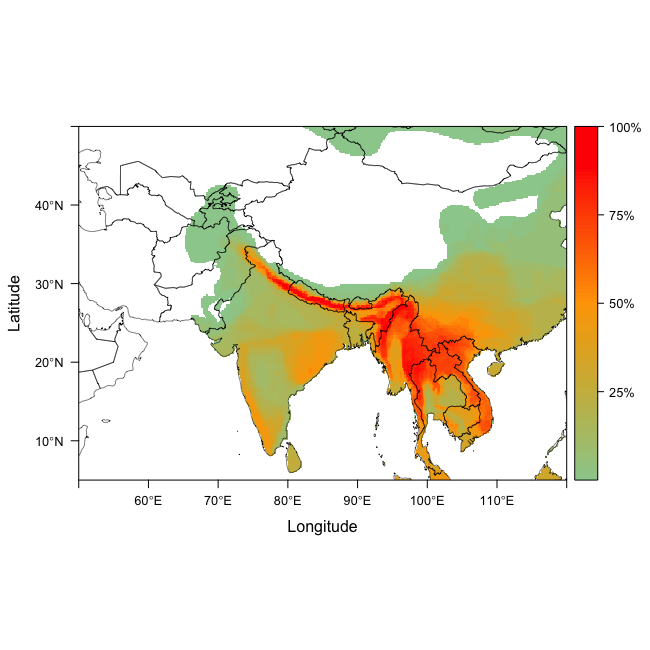
\includegraphics[width=6in,height=6in]{figure/maps.png}
\end{center}
\end{figure}



Finally, the user can generate the counts data corressponding to regional diversity using the \begin{verb} DispersionFieldTocounts() \end{verb} function

\begin{knitrout}
\definecolor{shadecolor}{rgb}{0.969, 0.969, 0.969}\color{fgcolor}\begin{kframe}
\begin{alltt}
\hlstd{regional_counts} \hlkwb{<-} \hlkwd{DispersionFieldToCounts}\hlstd{(dispersion.field)}
\end{alltt}
\end{kframe}
\end{knitrout}

\begin{knitrout}
\definecolor{shadecolor}{rgb}{0.969, 0.969, 0.969}\color{fgcolor}\begin{kframe}
\begin{alltt}
\hlkwd{dim}\hlstd{(regional_counts)}
\end{alltt}
\begin{verbatim}
## [1]     38 201600
\end{verbatim}
\begin{alltt}
\hlstd{regional_counts[}\hlnum{1}\hlopt{:}\hlnum{5}\hlstd{,}\hlnum{1}\hlopt{:}\hlnum{5}\hlstd{]}
\end{alltt}
\begin{verbatim}
##    [,1] [,2] [,3] [,4] [,5]
## U1    0    0    0    0    0
## U2    1    1    1    1    1
## MA    0    0    0    0    0
## A2    0    0    0    0    0
## A3    0    0    0    0    0
\end{verbatim}
\end{kframe}
\end{knitrout}


\subsection{functional motif}

In order to build counts data corresponding to functional diversity, we order the species based on some ordering metadata (like bill shape, size of the bird etc in our example). But there will be many zeros in the matrix as the species abundance data is sparse. To effectively account for the functional diversity and take into account the relatedness among the bird species, the zeros are filled in by kriging based on the species with non-zero abundance. We use the function \begin{verb} krige_counts \end{verb}.

\begin{knitrout}
\definecolor{shadecolor}{rgb}{0.969, 0.969, 0.969}\color{fgcolor}\begin{kframe}
\begin{alltt}
\hlstd{func_counts} \hlkwb{<-} \hlkwd{krige_counts}\hlstd{(taxonomic_counts,}
        \hlkwc{order} \hlstd{= species_metadata}\hlopt{$}\hlstd{bill_length,}
            \hlkwc{krige.control} \hlstd{=} \hlkwd{list}\hlstd{(}\hlkwc{cov.mod} \hlstd{=} \hlstr{"whitmat"}\hlstd{,} \hlkwc{sill}\hlstd{=}\hlnum{0.5}\hlstd{,} \hlkwc{smooth}\hlstd{=}\hlnum{.01}\hlstd{))}
\end{alltt}
\end{kframe}
\end{knitrout}

\begin{knitrout}
\definecolor{shadecolor}{rgb}{0.969, 0.969, 0.969}\color{fgcolor}\begin{kframe}
\begin{alltt}
\hlkwd{dim}\hlstd{(func_counts)}
\hlkwd{head}\hlstd{(func_counts[,}\hlnum{1}\hlopt{:}\hlnum{5}\hlstd{])}
\end{alltt}
\end{kframe}
\end{knitrout}


We can also use traits to collapse the bird species by performing hierarchical clustering of the bird species based on a single trait or multiple traits. We perform this using the `trait_cluster()` function in **ecostructure**. We demonstrate its application next.







